\chapter{A Compilation Example}
\label{chap:ACompilationExample}
This chapter firstly informally describes the \mbox{MiniML} source language (\myref{sec}{sec:MiniML}), a subset of the ML language whose syntax and semantics are reminiscent of those of Standard ML.
\myref{sec}{sec:MLExample} then introduces an example program (a Caesar cipher implementation) that will be used to show the secure compilation scheme.
This chapter continues by describing the LLVM intermediate language to which the first translation occurs (\myref{sec}{sec:LLVM}).
This chapter concludes by translating the earlier proposed example program, showing the resulting LLVM code (\myref{sec}{sec:translationexample}).
%The secure compilation scheme is shown from an example program written in the source language, \mbox{MiniML}, which is a subset of the ML language. Its syntax and semantics are reminiscent of those used in Standard ML.

\section{MiniML}
\label{sec:MiniML}
The ML language is a functional programming language that is well known for its module system.
This module system aims to group data and code together into coherent entities, called modules.

A \emph{structure} is the most basic type of module.
It can be defined using the \lsttext{struct} construct and provides a set of bindings for types, values and functions.
A structure specifies a name for the binding and the corresponding value, called \emph{implementation}.
Structures provide the possibility of grouping related code and data, fulfilling the need of \emph{modularization} in software.
However, the need for \emph{data abstraction} is not yet fulfilled.
\myref{lst}{code:DictionaryStructureExample} shows how a dictionary of strings to strings might be implemented by a module.
~
\begin{lstlisting}[frame=single, language=ML,caption={[Dictionary Definition Example]An example structure showing the definition of a dictionary in ML.}, label=code:DictionaryStructureExample,numbers=left]
structure Dictionary =
    struct
        type dictionary = (string * string) list
        val emptyDictionary = []
        fun insert d, x, y = (x,y)::d
    end
\end{lstlisting}

\myref{lst}{code:DictionaryStructureExample} firstly defines a type dictionary, which is defined to be a type synonym for a list of string pairs, a value representing the empty dictionary (\lsttext{emptyDictionary}) and a function for inserting data into the dictionary (\lsttext{insert}).

As it stands, the dictionary type is a type synonym for lists of string pairs, and any such list could be used where a dictionary is expected.
However, the concept of a dictionary does not require users to know that the dictionary type is implemented as a list of string pairs.
According to the principle of data abstraction, it is favorable to hide this information from the user of the dictionary module.

Here the idea of a signature comes into play.
A signature groups a set of types, values and functions without providing an implementation.
It provides a way of abstracting over structures that implement the same logical concept using a different implementation.
A possible signature for dictionaries is shown in \myref{lst}{code:SignatureDictionaryExample}.
~
\begin{lstlisting}[frame=single, language=ML, caption={[Dictionary Declaration Example]An example signature showing the declaration of a dictionary in ML.}, label=code:SignatureDictionaryExample, numbers=left]
signature DICTIONARYSIGNATURE =
    sig
        type dictionary
        val emptyDictionary : dictionary
        val insert: dictionary -> string -> string -> dictionary
    end
\end{lstlisting}

A signature guarantees that two implementations of the same logical concepts are interchangeable for each other by standardizing the way an implementation communicates with the other code.
It can also abstract the fact that the current implementation for dictionaries uses lists, as well as obscuring any helper methods that the specific implementation defines in order to simplify its internal workings.
This last functionality of a signature is a way to perform \emph{information hiding}.

%In order to simplify this study, the ML language is simplified to its core, resulting in the smaller \mbox{MiniML} language.
%This will, at first, only feature modules.
%Later on, It will be extended with more advanced concepts of ML, such as functors.

The \mbox{MiniML} fragment discussed here was chosen to incorporate only the idea of structures, more complex language features will be added later (\myref{chap}{chap:AdvancedConcepts}).

\section{A Cipher In \MiniML}
\label{sec:MLExample}
\myref{lst}{code:Example} presents a simple example program that consists of the definition of a signature that represents symmetric cyphers, a concept used in cryptography.
This example was chosen since the modules related to cryptography are usually under more scrutiny with regards to the privacy of their internal values.
The code in \myref{lst}{code:Example} defines a signature \lsttext{SYMMETRICCIPHER}.
This signature describes the common traits between modules that implement a symmetric cipher.
In order to implement a symmetric cipher, one must have a credential, i.e. the key, and two functions, \lsttext{encrypt} and \lsttext{decrypt}, which take data and credentials.
The \lsttext{encrypt} function takes the raw data and encodes it in a way only those with knowledge of the correct credentials can later use the \lsttext{decrypt} function to transform the encoded data back into the raw data.

\begin{lstlisting}[frame=single, language=ML,numbers=left, label=code:Example, caption={[Caesar Cipher Example]Example of a security sensitive module specifying and implementing a symmetric cypher.}]
signature SYMMETRICCIPHER =
    sig 
        type cred
        val newcredentials : cred
        val encrypt: int -> cred -> int
        val decrypt: int -> cred -> int
    end

structure Caesar :> SYMMETRICCIPHER =
    struct
        type cred = int
        fun newcredentials = rand
        fun encrypt a cred = (a + cred)%26
        fun decrypt a cred = (a - cred)%26
        val seed = 3
        fun rand = time.now * seed
    end
\end{lstlisting}

From line 8 of \myref{lst}{code:Example} onwards the definition of a structure called \lsttext{Caesar} is given.
\lsttext{Caesar} implements the \lsttext{SYMMETRICCYPHER} signature.
In this context, \lsttext{Caesar} provides the \lsttext{newcredential}, \lsttext{encrypt} and \lsttext{decrypt} functions.
For internal use it also possesses the necessary characteristics of a pseudorandom number generator, namely a seed value and a rand function that provides a pseudorandom number.
It is necessary to hide the seed value from users since this would allow attackers to predict the output of the pseudorandom number generator.

The \lsttext{Caesar} structure is forced to conform to the signature \lsttext{SYMMETRICCIPHER} by means of \emph{ascription}(\lsttext{:>}).
Ascription not only forces the module to implement all the necessary elements of the signature, but it also restricts the means of interaction with the module to those elements that are explicitly mentioned in the interface.
It is this notion of \emph{ascription} that dictates what it means for this module to be secure.

In this case, the ascription of the \lsttext{Caesar} structure with signature \lsttext{SYMMETRICCIPHER} is done opaque (\lsttext{:>}), as opposed to transparent (\lsttext{:}).
The difference between opaque and transparent ascription is as follows:
\begin{description}
\item[Opaque ascription] 
Ascribing a structure using opaque ascription \lsttext{:>} means any declaration, be it type or value, in the signature must have a corresponding definition in the structure.
The ascription hides any \lsttext{val} or \lsttext{fun} definition for which there is no corresponding \lsttext{val} declaration inside the signature.

For types declared in the signature, but without a specific implementation, the implementation of the type is unspecified.
In other words, for code outside the structure, the type and its implementation are not synonymous.
\item[Transparent ascription] 
Ascribing a structure using transparent ascription \lsttext{:} hides the same definitions as opaque ascription.

However, for types declared in the signature, but without a specific implementation, the implementation that the structure provides for the type is specified.
In other words, for code outside the structure, the type and its implementation are synonymous, and interchangeable.
\end{description}


Concretely, to be secure, this module hides its \lsttext{rand} function and its seed value from any outside code, only allowing the code internal to the structure to access this value or call the function.
Because the ascription is opaque, the implementation of \lsttext{cred} as an \lsttext{int} is hidden as well.
This makes it impossible for code outside the structure to use a value of type \lsttext{int} where a value of type \lsttext{cred} is expected, even though they are type synonyms inside the \lsttext{Caesar} structure.


\subsection{Compilation of \MiniML}
\label{sec:DefinitionOfCompilation}
Compilation of \MiniML\ reflects the compilation of the ML language.
As in ML, the \MiniML\ compilation process takes a \MiniML\ program as a collection of \emph{files} that contain signatures and structure definitions.
Conventionally, \MiniML\ processes each file in order of the collection, and separately, as a unit of compilation.

Within each file it processes the definitions in the order that they are listed in the file. It expects the resulting order in which it processes the definitions to correspond to a \emph{directed acyclic graph} or \emph{DAG}.
This means that a definition can only use elements that were defined \emph{before} its own definition.

When talking about the secure compilation of \MiniML, the remainder of this text will expect that a file containing all secure signature and structure definitions is passed to the compiler first.
This represents the secure module or \emph{SPM}, which contains all secure code.

Next, all code representing the context is compiled separately and later linked to the result of the compilation of the secure code.
%\todo{This is an important remark} 
As a result, the definitions of structures in secure code can not directly depend on elements that are defined only later, in the insecure context.

%This example can later be broadened so that the \lsttext{Caesar} structure becomes a functor that is parameterized to use an external module as its PRNG.

\section{LLVM and the LLVM Intermediate Representation}
\label{sec:LLVM}
This section introduces the LLVM and its intermediate representation.
It also specifies the expected LLVM intermediate representation code for the example in \myref{lst}{code:Example}.

\subsection{LLVM}
LLVM, short for \emph{Low Level Virtual Machine} is the name of a project providing many different and closely affiliated utilities concerned with the compilation process.
Created by Chris Lattner~\cite{Lattner} in 2000, the project was picked up by Apple and work on the LLVM project has continued up to this date.

The main sub-project of LLVM is the LLVM Core, which combines code generation and optimization for many platforms.
Because the generation of code for a specific platform and the optimization of code is generally very difficult work, the LLVM Core is built around the LLVM intermediate representation, or \LLVMIR.

This intermediate representation attempts to provide a shared abstraction that the compilers of many source-level languages can use.
The idea is that any source-level language can be compiled to the \LLVMIR, using the LLVM project as a \emph{backend} for its own compilation.
Once a source-level program is compiled to \LLVMIR, any form of optimization can be done on the LLVM intermediate representation, and thus optimizations are shared between the different source-level languages.

When all required optimizations are performed, it is possible to compile the intermediate language into machine code and perform linking of all necessary code.
Any special modification necessary to run on specific target platforms is shared across the 
different source languages as well, because the code generation uses the \LLVMIR\ as its input.

Providing a compiler for a source-level language is now confined to providing a compilation to the \LLVMIR.
When such a compiler exists, the full power of the LLVM optimizer is accessible for the source language, and compilation is possible to every one of the multitude of platforms compatible with LLVM.

\subsection{\LLVMIR}
%One of the important utilities being used in this work is LLVM's intermediate representation, 
This work uses LLVM as a \emph{backend}.
The secure compiler for \MiniML\ will translate \MiniML\ code into the LLVM intermediate representation.
In order to focus on the security of the compilation, the more aggressive optimization capabilities of LLVM will not be used.
\\[1em]
It is possible to write a program in this LLVM intermediate representation using one of three different and equivalent encodings, according to the \emph{LLVM Language Reference}~\cite{LLVMFAQ}:
\begin{itemize}
\item A bitcode format
\item Textual assembly language
\item A symbolic representation, manipulated by the LLVM API
\end{itemize}

This text will use the textual assembly language as representation for LLVM IR programs, because this makes examples and results more understandable and human readable.
While it is possible to generate LLVM IR programs using the LLVM API, this work chooses to generate the human readable intermediate code itself, because it offers more direct control over the resulting translation.

The benefit of LLVM intermediate representation is not limited to the points mentioned above.
The LLVM intermediate representation works at a higher level of abstraction than standard assembly does.
Some important additional aspects make the intermediate representation used by LLVM of a higher level of abstraction than standard assembly code:

\begin{description}
\item[Type System] More information about the program is captured by LLVM than when using regular assembly, using LLVM's type system.
This type system helps the optimalization process.

The type system, as given by the \emph{LLVM Language Reference}~\cite{LLVMFAQ} consists of the types shown in \myref{fig}{fig:llvmtypes}. Not all types are shown, the vector type and opaque types are omitted.

A shorthand for types can be defined using \lsttext{\%Name = type}.

\begin{figure}[htb]
\begin{tabularx}{\textwidth}{|l X|}
\hline
\multicolumn{2}{|c|}{\gray LLVM Basic Types}\\
iN & Arbitrary width integer. 
The width is specified by N. \\
Void & The void type. Like the void type in Java, this represents no value. The void value has no size.\\
\cmath{type\ast} & The pointer type. It specifies a specific memory location. The memory location must contain a value with the correct type, as specified by \cmath{type}. It is considered by the \emph{LLVM Language Reference} to be a basic type.\\
label & The label type. This specifies a pointer to a label. This is equivalent to i8*.\\
\multicolumn{2}{|c|}{\gray LLVM Derived Types}\\
\cmath{[}N x \cmath{type}\cmath{]} & The Array type. This represents N elements of type \cmath{type} ordered sequentially in memory.\\
\{\cmath{type list}\} & The structure type. This represents a sequence of values in memory of type \cmath{type}. The elements are in the order of the list. The list is comma separated.\\
\cmath{type_{1}}(\cmath{type list}) & The function type. This represents a function that returns a value of type \cmath{type_{1}}, and takes arguments with the types specified in the type list.\\
\hline
\end{tabularx}
\caption[LLVM Types]{The LLVM types, with vector types and opaque types omitted. \label{fig:llvmtypes}}
\end{figure}

\item[Register Limitations]  The LLVM intermediate representation abstracts away the fact that real architectures have only a given amount of registers.
Instead, one can write a program assuming an infinite amount of \emph{virtual registers}.
This results in many more variables in use than available registers.
In a later compilation stage this consequence is remedied using the technique of \emph{spilling}.
Variable spilling occurs by mapping the variables in use to the smaller set of available registers, saving all variables that could not be assigned to a register in RAM memory in the stack.

\item[SSA] For optimization purposes, the LLVM IR adheres to the \emph{static single assignment} paradigm, or \emph{SSA}.
This implies that every register can be assigned a value only once.

For example, the code in \myref{lst}{lst:reassign} reassigns the value saved in register x from 3 to  4. In SSA, this would be represented by \myref{lst}{lst:ssa}.
\begin{lstlisting}[label=lst:reassign, caption={[Variable Reassignment]Reassigning a variable.}, frame=single, language={[x86masm]Assembler}]
Block:
    %x = 3;
;    br i1 %cond, label %Cond, label %Ret
Cond:
    %x = add i32 %x, 1;
Ret:
    ret i32 %x;
\end{lstlisting}

\begin{lstlisting}[label=lst:ssa, caption={[SSA Representation 1]Code in SSA form.}, frame=single, language={[x86masm]Assembler}]
Block:
    %x1 = 3;
;    br i1 %cond, label %Cond, label %Ret
Cond:
    %x2 = add i32 %x1, 1;
Ret:
    ret i32 %x2;
\end{lstlisting}
This essentially provides a versioning postfix to the variable identifier. 
%Since all registers in \LLVMIR\ are virtual registers, an infinite amount is available.
%As a result, this versioning method is 
The problem with SSA becomes worse however if the modification of x depends on control flow. For example by uncommenting the conditional statement in \myref{lst}{lst:reassign}, the eventual value of \lstinline[language={[x86masm]Assembler}]{\%x} depends on the value of \lstinline[language={[x86masm]Assembler}]{\%cond}.

The return statement in \myref{lst}{lst:ssa} should now return either \lsttext{\%x1} or \lsttext{\%x2}.
But how can the code in SSA form decide which of the two registers should be returned?
LLVM IR solves this problem by providing the $\Phi$ function~\cite{Appel}.

The $\Phi$ function `merges' a set of variables.
It assigns a new variable the value of one of a number of old values, where the choice of the old value depends on the control flow.
In \myref{lst}{lst:ssaphi}, the SSA-representation of \myref{lst}{lst:reassign} with the condition uncommented is shown.

\begin{lstlisting}[label=lst:ssaphi, caption={[SSA Representation 2]Code in SSA form with function.}, frame=single, language={[x86masm]Assembler}]
Block:
    %x1 = 3;
    br i1 %cond, label %Cond, label %Ret

Cond:
    %x2 = add i32 %x1, 1;
    
Ret:
    %x3 = phi i32 [%x1 Block] [%x2 Cond]
    return %x3;
\end{lstlisting}

%First, this restriction poses no real hindrance to a functional language as \MiniML, which already is single assignment.
%This restriction is solved by providing the $\Phi$ function~\cite{Appel} as a way to write code that modifies a registers value.

%\to do{This is important for the secure compilation (clearing registers after function calls end). It might be necessary to rework this subsection to stress this more.}
\end{description}

\subsection{Translating \MiniML\ concepts to LLVM}
\label{sec:translation}
Compiling from \MiniML\ to LLVM IR means the high-level abstractions made in \mbox{MiniML}, for example \emph{signatures} and \emph{structures}, must be mapped to lower-level constructs that are available in the LLVM intermediate representation.
This section presents these different mappings.

\begin{description}
\item[File]
A file with ML structures and signatures inside it is a separate unit of compilation.
Its signatures and structures are type checked and compiled together. 
When a file is compiled, there can only be dependencies on values that were defined in an earlier unit of compilation, since the compilation of \MiniML\ expects a directed acyclic graph, as explained in \myref{sec}{sec:DefinitionOfCompilation}.

LLVM already provides the concept of a module as a separate unit of compilation.
This means each LLVM module is compiled to a single different object file.
Firstly, an LLVM module declares which external functions will be provided by other code, and then continues by defining and implementing its own code and data.
These definitions and external references are compiled into a single object file.
LLVM poses no restrictions on the access of data and functions within a single module.
This is poses no problem for files containing multiple secure structures. Since they are first type checked together before being compiled together, a secure structure will never access a hidden component of another secure structure.

The access of data and functions from within other modules \emph{is} restricted by LLVM: the object file to which a module is compiled is accompanied by a link table.
This link table specifies which methods are defined and made externally visible, which is used to match the declaration of external functions with their implementation in other object files.
The link tables represent what other code knows about the definitions contained within the compiled module.


\item[Structures]
Structures are a collection of types and value definitions.
As such they can be compiled by compiling every one of their components.

Structures also provide namespaces: 2 structures str$_{1}$ and str$_{2}$ can both define a value t without resulting in a clash of names.
When compiling structures by compiling every one of their components, this situation should not introduce a clash of names either.
This is guaranteed by identifier prefixing: When a component $x$ within str$_{1}$ is compiled, the compilation is not bound to $x$ but to str$_{1}.x$ instead.


%LLVM already provides the concept of a module as a separate unit of compilation. This means each LLVM module is compiled to a single different object file. Firstly, an LLVM module declares which external functions will be provided by other code, and then continues by defining and implementing its own code and data. These definitions and external references are compiled into a single object file. LLVM poses no restrictions on the access of data and functions within a single module, but in order to manage the access of data and functions from within other modules, the object file to which a module is compiled is accompanied by a link table specifying which methods are defined and made externally visible, which is used to match the declaration of external functions with their implementation in other object files. The link tables represent what other code knows about the definitions contained within the compiled module.

%This means that LLVM already provides a way of performing code and data encapsulation.

%  When compiling these modules the result is a single object file. Each of these object files is accompanied by a.

%The functionality offered by LLVM IR modules makes them the right target  to map the different ML structures onto.

\item[Functions]
LLVM provides the concept of a function as a set of basic blocks of code. 
These LLVM IR functions allow the programmer to modify the visibility of a function using the linkage keyword. 
%The concept of a function as a basic building blocks allows us to specify the visibility of these blocks towards outside code. 

When linking the object files that result from the compilation of different modules, LLVM looks for the implementation of externally declared functions in the different object files, keeping into account whether or not the code was in fact declared to be visible outside the module. It is possible to map ML functions directly to their LLVM counterpart.

\item[Signatures]
While structures can be mapped directly onto the concept of a module in LLVM, the information provided in signatures will mainly affect metadata in the resulting code or influence the specific implementation of different elements inside the modules.

When a structure is opaquely ascribed, or \emph{sealed} by a signature, we must make sure that the values and functions defined in the structure but not specified in the signature are not externally visible. The first step in protecting these internal functions consists of marking these members as private in the module corresponding to the ML structure. This will filter these members from the object files link table. %This way these private members are protected from access by any of the external code generated by the same compiler.

%Structures will be mapped onto the different modules, while the information provided in the signatures will mainly affect metadata in the resulting code, or influence the specific implementation of different elements inside the modules.

\item[Value]
The translations of a value is a getter function without arguments.
This is necessary because \begin{itemize}
 \item The value might not be defined as a constant, but as the result of a call to a pure function.
 This does not violate the constraint that a value must represent an immutable value, because the result of a pure function call will always result in the same result. 
When translated, this function must be executed however and the result must be passed.
\item These values are readable by any code.
As shown later, when it is read by the insecure context, certain precautions must be taken.
This is impossible when values are translated to constants.
 \end{itemize}

%Translations of the fields happens as global constants within a module. Since their value is unchanging, the \emph{SSA} paradigm poses no real limitation.

\end{description}

\section{Translation Example: The Caesar Cipher}
\label{sec:translationexample}
In order to study the compilation scheme, the example ML code in \myref{lst}{code:Example} is translated to LLVM IR.

The code given to the compiler is treated as a single file containing all secure or trusted structures.
In the case of \myref{lst}{code:Example}, this consists of only the \lsttext{Caesar} structure.
As mentioned in \myref{sec}{sec:translation}, this is compiled to a single LLVM module.

Before discussing the translation of \myref{lst}{code:Example}, the security concerns that MiniML introduces have to be discussed.

\subsection{MiniML-specific security concerns}
\label{sec:securityconcerns}

\subsubsection{Ordering of Fields and Module Expressions}
The necessity of reordering field definitions in a target-level object was shown by Agten et al.~\cite{Agten:2012:SCM:2354412.2355247}.
In \MiniML\ the same argument holds, not only for fields, but for the order of structure definitions as well.

The order in which structures and signatures are defined, or the order of fields within a structure is to a large extent unimportant for the behavior of a \MiniML\ program.
As long as no structure is used before it is defined, differently ordered \MiniML\ programs are contextually equivalent.
The order of field definitions within a structure has no result on the behavior of the program either.

The ordering of structure or field definitions in \LLVMIR\ might be leaked however, when examining the pointers to different fields.
If contextually equivalent but differently ordered \MiniML\ programs would be translated to differently ordered \LLVMIR\ programs, the results would not be contextually equivalent.

To guarantee \emph{full abstraction}, it is thus necessary to ensure that all contextually equivalent but differently ordered \MiniML\ programs result in the same ordering of definitions in \LLVMIR.
This can be accomplished by alphabetically ordering structures, and the fields within their structures, when outputting the \LLVMIR\ program.

\subsubsection{Stack Switching}
As described by Agten et al.~\cite{Agten:2012:SCM:2354412.2355247}, when code execution switches from protected code to unprotected code or back, the security of the run-time stack must be protected.
Therefore the stack is split into two parts, the secure stack and the insecure stack.
These are respectively located in secure and insecure memory.
The following precautions, as described by Agten~\cite{Agten:2012:SCM:2354412.2355247} are then taken:
\begin{itemize}
\item When the secure code is entered in an entry point, the stack pointer is modified to point to the secure stack, whose location is saved in a field in the data section.
This field is called the \emph{shadow stack pointer}.
There is another field reserved in the data section as well, to keep track of the value of the stack pointer before modification.
\item At each exit point, the stack is restored to its previous
address in unprotected memory, and the location of the \emph{shadow stack pointer} is updated.
\end{itemize}

Because this is only necessary when functions are called from the unprotected code, these security measures are taken care of by a low-level stub that wraps around the low-level translation the high-level publicly available function.
%every publicly available function is made available through a publicly available stub which will take care of these security measures.
This stub will then forward execution to an internal function (which is not publicly available) which will strictly focus on the low-level implementation of the high-level function itself.
This internal function can thus assume that any necessary security precautions are taken.
Within the secure code, calls to these internal functions can happen directly, without passing through the stub.
%It assumes the necessary security precautions are taken, and can be used directly within the secure code.

\subsubsection{Register Clearing}
Any communication in \mbox{MiniML} normally only occurs through information passed along by returns and method calls.
In the case of low-level architecture however, all communication occurs through the unprotected memory, through flags and through the CPU registers.
This means that a low-level attacker can try to perform side channel communication.

In order to prevent the leaking of protected data through side channels, it is important to ensure that the information passed through unprotected memory, flags and registers is restricted to that information being passed by the returns and method calls in \mbox{MiniML}.
Thus, any callback or return to untrusted code must: %~\cite{Agten:2012:SCM:2354412.2355247}:
\begin{itemize}
\item Clear the flags
\item Clear the registers, except those being used to pass a parameter or a return value.
\end{itemize}

If these registers and flags, which were possibly modified by the protected code, are not reset when returning execution to unprotected memory, code running in the unprotected memory will be able to read the values in these registers and flags, breaking confidentiality. The code could even modify these values, resulting in a modification of control flow if execution is later returned to the protected code while expecting these values to be uncorrupted.

However, since the LLVM intermediate representation does not allow multiple assignments to the same registers, it is impossible to clear a register simply by overwriting its value.
Furthermore, the LLVM IR does not know how many registers it can use, instead assuming an infinite amount of registers, as mentioned earlier. This means that clearing these registers must happen later on in the compilation process, introducing an extra LLVM pass.

This clearing can once again happen inside the stub, keeping the internal functions free from any code related to security concerns.

\subsubsection{Opaque types}

The \mbox{MiniML} language allows a programmer to define his own types using the type keyword. Taking another look at the Dictionary example of \myref{lst}{code:DictionaryStructureExample}, this happens in line 3. The modules internal representation of a dictionary is a list of string pairs, but clearly this is some internal choice that the programmer does not want to make explicit, which is why the type synonym \lsttext{dictionary} is kept opaque, as can be seen in \myref{lst}{code:SignatureDictionaryExample}, line 3, where the external specification of a type is not revealed to be a list of string pairs.

This is a means of information hiding, if someone were to later rewrite this dictionary structure in such a way that its internal representation changes, e.g. it becomes a pair of string lists as in \myref{lst}{code:DictionaryStructureExample2}, this would be a perfectly valid change. This change should not result in any changes to the external code, since the specific implementation choice for the dictionary type was not made explicit.

\begin{lstlisting}[frame=single, language=ML, label={code:DictionaryStructureExample2},caption={[Alternative Dictionary Definition]An alternative structure defining a dictionary.}]
structure Dictionary =
    struct
        type dictionary = (string list * string list)
        val emptyDictionary = ([],[])
        fun insert((fst,snd), x, y) = (x::fst, y::snd)
    end
\end{lstlisting}

Even more so, one would expect the two programs/modules to be contextually equivalent! However, clearly, if no checking is performed within functions expecting something of type dictionary, a low-level attacker could discriminate between the two using the following tactic: call a function expecting a dictionary argument with a self-created list of string pairs. If it gives the expected results, the dictionary implementation being used is the one given in \myref{lst}{code:DictionaryStructureExample}. If not, it is the module described in \myref{lst}{code:DictionaryStructureExample2}, expecting a pair of string lists. This breaks contextual equivalence.

The code must assure that any object, passing as an argument of type dictionary, was in fact created by the module code itself (using the \lsttext{emptydictionary} method). If not, it should raise an error (even if the object has the correct type according to the synonyms) in order to prevent an attack on contextual equivalence in the same spirit as the one described above.

This restriction can be enforced by a technique called masking, introduced by Patrignani et al.~\cite{Patrignani}. 
Masking works by ensuring that the code creating a dictionary never returns a pointer to this dictionary itself, instead saving this dictionary pointer in an internal list located within protected memory.
The index in this list can then be returned and used as a mask for the real object.
Once again, this masking can be done within the stub function that wraps around the internal function that returns the value.

When a stub represents a high level function that expects an argument of an opaque type, it will receive the index of the desired value in the internal masking list.
It can use the internal masking list to retrieve the pointer associated with the index, and to check whether it points to a value of the right type.
%The technique of masking and unmasking in the security boundary is visualized in \myref{fig}{fig:Masking}, which shows that the regular pointer is used within protected memory, but that is masked and unmasked by stubs when passing through the boundary.
%
%\begin{figure}
%\centering
%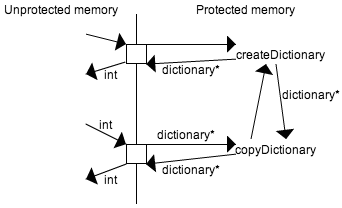
\includegraphics[scale=0.5]{img/Masking.png}
%\caption{Visual representation of the masking technique. \label{fig:Masking}}
%\end{figure}


\subsubsection{Entry points}
Instructions in the insecure code can only jump to memory locations marked as an entry point by the \emph{SPM}'s metadata.
This compilation scheme adds an entry point to the \emph{SPM} for every function available in the high-level language.
Because the security checks are performed inside the stubs, it might seem logical to use the memory locations of their first instructions as the entry points for the \emph{SPM}.

However, because the size of these functions can be derived from the distance between two successive entry points, and this size might leak information about the \emph{SPM}, the memory locations of these stubs are not listed as entry points.
Instead, a small entry function that calls these stubs is created, in the low-level this corresponds to a simple tail call.
These small entry functions can be grouped together in the secure code section, and take up a constant amount of space.
The memory locations corresponding to these entry functions can then be listed in metadata as entry points for the \emph{SPM}.

%All public available low-level functions (i.e. the stubs that represent public high-level functions) that expect a dictionary as their argument then no longer get a pointer to this dictionary object in memory. 
%Instead, they get the index of the desired dictionary in the internal list.

%When these publicly available functions receive the index, they get the pointer associated with the index from the internal list and check whether it points to the right type of object.
%
%
%\todo{The explanation of why extra type information might prove necessary. However: The argument must be presented in a more careful manner. Furthermore, this also depends on whether a separate list is being used per type or not. If a separate list is being used anyway, instead of a central list of masked objects, then the extra type information proves unnecessary, or rather, it is already implicitly available.}

\subsection{Translation}
\label{sec:TranslatedExample}
The translation to LLVM intermediate representation is given in code in \myref{lst}{llvm:Example}.

\begin{lstlisting}[frame=single,numbers=left, language={[x86masm]Assembler}, caption={[LLVM Translation Caesar Cipher Example]LLVM IR for the example.},
label=llvm:Example]
%int = type i64
%Caesar.cred = type {%int} ±\label{ln:cred_type_def}±

declare i8* @malloc(%int)
declare void @free(i8*)
declare void @exit(i32)

define %int @Caesar.decrypt(%int %arg0, %int %arg1) { ±\label{ln:decrypt_entry_start}±
   %ret = tail call %int @Caesar.decrypt_stub(%int %arg0, %int %arg1)
   ret %int %ret
} ±\label{ln:decrypt_entry_end}±

define %int @Caesar.encrypt(%int %arg0, %int %arg1) { ±\label{ln:encrypt_entry_start}±
   %ret = tail call %int @Caesar.encrypt_stub(%int %arg0, %int %arg1)
   ret %int %ret
} ±\label{ln:encrypt_entry_end}±

define private %int @Caesar.newcredentials() { ±\label{ln:newcredentials_entry_start}±
   %ret = tail call %int @Caesar.newcredentials_stub()
   ret %int %ret
} ±\label{ln:newcredentials_entry_end}±

define private %int @Caesar.decrypt_stub(%int %arg0, %int %arg1) noinline { ±\label{ln:decrypt_stub_start}±
   %arg1int = call %int @unmask(%int %arg1)
   %arg1type = call %int @unmasktype(%int %arg1)
   %check1 = icmp eq %int %arg1type, 4
   br i1 %check1, label %Continue, label %Error
   
   Continue:
   %arg1ptr = inttoptr %int %arg1int to %Caesar.cred*
   %ret = call %int @Caesar.decrypt_internal(%int %arg0, %Caesar.cred* %arg1ptr)
   ret %int %ret
   
   Error:
   call void @exit(i32 -1)
   unreachable
} ±\label{ln:decrypt_stub_end}±

define private %int @Caesar.decrypt_internal(%int %a, %Caesar.cred* %credptr) { ±\label{ln:decrypt_internal_start}±
   %loccred = getelementptr inbounds %Caesar.cred* %credptr, i32 0, i32 0
   %cred = load %int* %loccred 
   %x = sub %int %a, %cred
   %y = urem %int 26, %x 
   ret %int %y
}±\label{ln:decrypt_internal_end}±

define private %int @Caesar.encrypt_stub(%int %arg0, %int %arg1) noinline { ±\label{ln:encrypt_stub_start}±
   %arg1int = call %int @unmask(%int %arg1)
   %arg1type = call %int @unmasktype(%int %arg1)
   %check1 = icmp eq %int %arg1type, 4
   br i1 %check1, label %Continue, label %Error
   
   Continue:
   %arg1ptr = inttoptr %int %arg1int to %Caesar.cred*
   %ret = call %int @Caesar.encrypt_internal(%int %arg0, %Caesar.cred* %arg1ptr)
   ret %int %ret
   
   Error:
   call void @exit(i32 -1)
   unreachable
}±\label{ln:encrypt_stub_end}±

define private %int @Caesar.encrypt_internal(%int %a, %Caesar.cred* %credptr) {±\label{ln:encrypt_internal_start}±
   %loccred = getelementptr inbounds %Caesar.cred* %credptr, i32 0, i32 0
   %cred = load %int* %loccred
   %x = add %int %a, %cred
   %y = urem %int 26, %x
   ret %int %y
}±\label{ln:encrypt_internal_end}±

define private %int @Caesar.newcredentials_stub() noinline { ±\label{ln:newcredentials_stub_start}±
   %credptr = call %Caesar.cred* @Caesar.newcredentials_internal() ±\label{ln:newcredentialscall}±
   %credint = ptrtoint %Caesar.cred* %credptr to %int
   %ret = call %int @mask(%int %credint,%int 4)
   ret %int %ret
}±\label{ln:newcredentials_stub_end}±

define private %Caesar.cred* @Caesar.newcredentials_internal(){±\label{ln:newcredentials_internal_start}±
   %rand = call %int @Caesar.rand()
   %ptr1 = call i8* @malloc(%int 16)
   %ptr = bitcast i8* %ptr1 to %Caesar.cred*
   %locval = getelementptr inbounds %Caesar.cred* %ptr, i32 0, i32 0
   store %int %rand,%int* %locval
   ret %Caesar.cred* %ptr
}±\label{ln:newcredentials_internal_end}±

define private %int @Caesar.rand_internal() { ±\label{ln:rand_internal_start}±
   %t = call %int @Caesar.seed()
   ret %int %t
}±\label{ln:rand_internal_end}±

define private %int @Caesar.seed_internal() { ±\label{ln:seed_internal_start}±
   ret %int 3
}±\label{ln:seed_internal_end}±
\end{lstlisting}

This code, that implicitly is part of a module, consists of a list of \emph{global values}, denoted by the @ sign.
Every value, be it a global function or a global variable, has a \emph{linkage} type associated with it.
Linkage types control the accessibility of of variables and functions. The two linkage types in use are \lsttext{private}, which makes a value only accessible by objects inside the same module, and the default linkage type, \lsttext{external}.

The code in \myref{lst}{llvm:Example} specifies 11 different global values, corresponding to the 5 definitions in the \lsttext{Caesar} structure, their three stubs and the three entry functions. It also defines one type, corresponding to the \lsttext{cred} type.
As mentioned earlier, the ordering of these functions is alphabetical.
\begin{description}
\item[cred type] To start the translation, a type definition for the \lsttext{cred} type is given on line~\myref{ln}{ln:cred_type_def}.
It is represented as a structure, where first the effective structure is represented, and then an \lsttext{\%int} is reserved to keep track of the type.
Here, the number 4 is chosen to correspond with the \lsttext{cred} type.

\item[encrypt \& decrypt] The first translated functions are the \lsttext{encrypt} en \lsttext{decrypt} functions. The translation starts with the definition of \lsttext{@Caesar.decrypt_internal} on line~\myref{ln}{ln:decrypt_internal_start} in the code of \myref{lst}{llvm:Example}, and that of \lsttext{@Caesar.encrypt_internal} on line~\myref{ln}{ln:encrypt_internal_start}.
Both definitions use linkage type private.

Since these functions are available in ML for untrusted code, stubs are provided where security precautions can be made. These can be found on lines~\myref{ln}{ln:decrypt_stub_start}-\myref{ln}{ln:decrypt_stub_end} and \myref{ln}{ln:encrypt_stub_start}-\myref{ln}{ln:encrypt_stub_end}.
The definitions of these stubs take only \lsttext{\%int} values as arguments: these are either real integer values, or masked indices.

The stubs are marked as private as well, and entry point functions are created that perform a tail call to these stubs. These can be seen on lines~\myref{ln}{ln:decrypt_entry_start}-\myref{ln}{ln:decrypt_entry_end} and \myref{ln}{ln:encrypt_entry_start}-\myref{ln}{ln:encrypt_entry_end}.
These entry points specify no linkage type explicitly, which means linkage type \lstinline[language={[x86masm]Assembler}]{external}  is used.

When calling these functions from insecure code, execution starts at the entry functions, as their memory locations are listed as entry points by the \emph{SPM}.
These entry functions perform a tail call to the stubs.

The stubs know that the second argument to the internal function must be of type \lsttext{\%Caesar.cred*}, so they use the \lsttext{@unmask} function to get the corresponding \lsttext{\%Caesar.cred*} value, and type check it.

The definitions of the internal functions take one \lsttext{\%int} and one \lsttext{\%Caesar.cred*} as argument.
They can read the integer value that this \lsttext{cred} represents by accessing the representation, using the \lsttext{getelementptr} function in combination with the pointer \lsttext{\%Caesar.cred*}.

The body of the internal function uses the effective values in two calls to arithmetical assembly functions and returns the result.

\item[newcredentials] Next is the \lsttext{newcredentials} function.
An entry function for this publicly available function is defined on lines~\myref{ln}{ln:newcredentials_entry_start}-\myref{ln}{ln:newcredentials_entry_end}, performing a single tail call to the stub.
On lines~\myref{ln}{ln:newcredentials_stub_start}-\myref{ln}{ln:newcredentials_stub_end} in the code of \myref{lst}{llvm:Example}, a stub for the function is defined and its return type is declared to be \lsttext{\%int}, since it returns an index in the masking list.

On line~\myref{ln}{ln:newcredentialscall}, the stub calls the internal function, which returns a pointer value of type \lsttext{\%Caesar.cred*}.
The stub casts this pointer to an \lsttext{\%int}, and saves the \lsttext{\%int} as well as type information in the masking list using a call to \lsttext{@mask}.
This returns an index which can be returned to the context.

%This proxy acts as a wrapper around the real translation of \lsttext{newcredentials} that can be seen on lines 6-9. This proxy is the entry point to the function that is made available to the untrusted code. This proxy can perform the security precautions that have to be taken when taking values from or returning values to the untrusted code.

The body of the internal function \lsttext{@Caesar.newcredentials\_internal} implements the functionality of the ML \lsttext{newcredentials} function.
\lsttext{@Caesar.newcredentials\_internal} performs a call to the rand function, saving the resulting return value and creating a pointer to it.
This pointer is returned.

\item[rand] The function \lsttext{rand} is defined starting line~\myref{ln}{ln:rand_internal_start} and onwards in \myref{lst}{llvm:Example}.
As the structure \lsttext{Caesar} is opaquely ascribed by the signature \lsttext{SYMMETRICCIPHER}, and the value \lsttext{rand} is not specified in this signature, it should be hidden from any outside components.
This means the linkage type is set to \lsttext{private}
It also follows that no stub nor entry function is necessary for the \lsttext{seed} function.

In its body, it returns the value of the seed.

\item[seed] The value \lsttext{seed} is translated to a getter function.
For the same reasons as the variable \lsttext{rand}, its linkage type is set to \lsttext{private}. 

The definition of \lsttext{seed} can be seen on lines~\myref{ln}{ln:seed_internal_start}-\myref{ln}{ln:seed_internal_end} in the code of listing~\myref{lst}{llvm:Example}.
\end{description}

\section{Lessons learned}

This chapter gave an introduction to the \mbox{MiniML} language, which was chosen because of its special module system and how it specifies security aspects. Formalizing the \mbox{MiniML} language semantics will be the topic of \myref{chap}{chap:formalspecification}.

Furthermore, LLVM and its intermediate representation was introduced as the target language for the described compilation scheme.

The chapter proceeded by describing the compilation scheme, showing how \emph{structures} can be mapped to LLVM \emph{modules}, followed by a translation of its \emph{fields} and \emph{functions} to global variables and LLVM \emph{functions}.

\emph{Signatures} were shown to have no translation to a single LLVM concept, instead having an influence on the translation of the modules that it \emph{seals} in linkage types and more subtle ways.

The chapter concluded with a discussion about preventing side channel communication, which makes it necessary to clear registers and flags when calling or returning to any external code.

The existence of opaque types in \mbox{MiniML} means that objects of these opaque types can only be created by methods inside the module that declares the type synonym. To ensure this, the use of masking and the tracking of type information proved necessary.
